\section{Preventivo}
	\subsection{Dettaglio attività}
		\textcolor{red}{assicurarsi che sia temrine giusto. cookies avevano messo "fase" ma tv li ha rektati}
		\subsubsection{Analisi dei Requisiti di Massima}
			\paragraph{Suddivisione lavoro} \Spazio
			Nell'attività di \textit{Analisi dei Requisiti di Massima} ciascun componente del gruppo andrà a rivestire i seguenti ruoli:
			\begin{table}[H]
				\centering
				\begin{tabular}{C{4cm}|C{0.6cm}|C{0.6cm}|C{0.6cm}|C{0.6cm}|C{0.6cm}|C{0.6cm}|C{3cm}}
					\hlineB{3}
				\thead{Nominativo} &\thead{Re} &\thead{Am} &\thead{An}&\thead{Pt}&\thead{Pr}&\thead{Ve}&\thead{Ore totali}\\
					\hlineB{3}
					Paolo Eccher & - & - & - & - & - & - & - \\
					Alberto Gallinaro & - & - & - & - & - & - & - \\
					Giuseppe Merlino & - & - & - & - & - & - & - \\
					Elia Montecchio & - & - & - & - & - & - & - \\
					Lisa Parma & - & - & - & - & - & - & - \\
					Francesco Parolini & - & - & - & - & - & - & - \\
					Davide Zago & - & - & - & - & - & - & - \\
					\textbf{Ore totali ruolo}  & \textbf{-} & \textbf{-} & \textbf{-} & \textbf{-} & \textbf{-} & \textbf{-} & \textbf{-} \\
					\hlineB{3}
				\end{tabular}
				\caption{Suddivisione del lavoro - \textit{Analisi dei Requisiti di Massima}}	
			\end{table}
			
			Tali dati sono riassunti graficamente nel seguente diagramma a barre:
			
			\textcolor{red}{METTERE DIAGRAMAM}		
			
			\paragraph{Prospetto economico} \Spazio
			Nello svolgimento di questa attività i costi sostenuti per ogni ruolo, non a carico del proponente trattandosi dell'investimento iniziale, sono riassunti nella seguente tabella:
			\begin{table}[H]
				\centering
				\begin{tabular}{p{4cm}|C{4cm}|C{4cm}}
					\hlineB{3}
					
					\thead{Ruolo} &\thead{Ore previste} &\thead{Costo}\\
					
					\hlineB{3}
					Responsabile & 29 & 870,00\euro \\
					\hline
					Amministratore& 18 & 360,00\euro \\
					\hline
					Analista & 61 & 1.525,00\euro \\
					\hline
					Progettista & - & 0\euro \\
					\hline
					Programmatore & - & 0\euro \\
					\hline
					Verificatore & 46 & 690,00\euro \\
					\hline				
					\textbf{Ore totali} & \textbf{154} & \textbf{3.445.00 \euro} \\
					\hlineB{3}
				\end{tabular}
				\caption{Costi per ruolo - \textit{Analisi dei Requisiti di Massima}}
			\end{table}

			
			La suddivisione delle ore di lavoro tra i vari ruoli è raffigurata graficamente attraverso il seguente diagramma circolare:
			\begin{figure}[h] 
			\centering 
				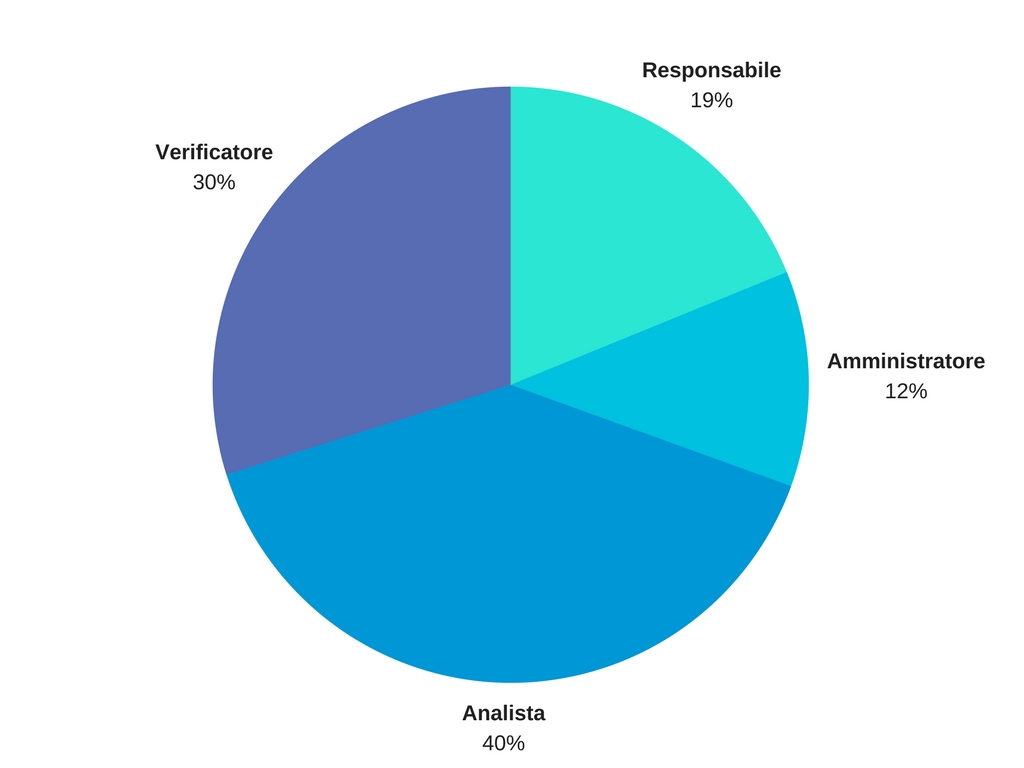
\includegraphics[width=0.9\textwidth]{images/CircolareAnalisiRequisitiDiMassima.jpg} 
				\caption{Diagramma circolare ripartizione ore per ruolo in Analisi dei Requisiti di Massima}
			\label{CircolareAnalisiRequisitiDiMassima}
			\end{figure}

			
			Come precedentemente detto nella sezione 3.1.2 di questo documento nel periodo di attesa dell'esito di questa attività ogni componente del grupo dovrà impegnare 10 ore in attività di approfondimento e studio delle tecnologie utili ai fini del profetto. Questo impegno non sarà rendicontato al proponente, nè ne sarà fornita una stima di costo in quanto non è assimilabile a nessun ruolo di progetto.
		
		\subsubsection{Analisi dei Requisiti di Dettaglio}
			\paragraph{Suddivisione lavoro}
			Nell'attività di \textit{Analisi dei Requisiti di Dettaglio} ciascun componente andrà a rivestire i seguenti ruoli:
			\begin{table}[H]
				\centering
				\begin{tabular}{C{4cm}|C{0.6cm}|C{0.6cm}|C{0.6cm}|C{0.6cm}|C{0.6cm}|C{0.6cm}|C{3cm}}
					\hlineB{3}
					\thead{Nominativo} &\thead{Re} &\thead{Am} &\thead{An}&\thead{Pt}&\thead{Pr}&\thead{Ve}&\thead{Ore totali}\\
					\hlineB{3}
					Paolo Eccher & - & - & - & - & - & - & - \\
					Alberto Gallinaro & - & - & - & - & - & - & - \\
					Giuseppe Merlino & - & - & - & - & - & - & - \\
					Elia Montecchio & - & - & - & - & - & - & - \\
					Lisa Parma & - & - & - & - & - & - & - \\
					Francesco Parolini & - & - & - & - & - & - & - \\
					Davide Zago & - & - & - & - & - & - & - \\
					\textbf{Ore totali ruolo}  & \textbf{-} & \textbf{-} & \textbf{-} & \textbf{-} & \textbf{-} & \textbf{-} & \textbf{-} \\
					\hlineB{3}
				\end{tabular}
				\caption{Suddivisione del lavoro - \textit{Analisi dei Requisiti di Dettaglio}}
			\end{table}
			
			Tali dati sono raissunti nel seguente diagramma a barre:
			
			\textcolor{red}{METTERE DIAGRAMAM}

			\paragraph{Prospetto economico}
			Nello svolgimento di questa attività i costi sostenuti per ogni ruolo sono raissunti nella seguente tabella:
			\begin{table}[H]
			\centering
			\begin{tabular}{p{4cm}|C{4cm}|C{4cm}}
				\hlineB{3}
				
				\thead{Ruolo} &\thead{Ore previste} &\thead{Costo}\\
				\hlineB{3}			
				Responsabile & 9 & 270,00\euro \\
				\hline
				Amministratore& 3 & 60,00\euro \\
				\hline
				Analista & 17 & 425,00\euro \\
				\hline
				Progettista & - & 0\euro \\
				\hline
				Programmatore & - & 0\euro \\
				\hline
				Verificatore & 13 & 195,00\euro \\
				\hline
				\textbf{Ore totali} & \textbf{42} & \textbf{950.00 \euro} \\
				\hlineB{3}
			\end{tabular}
			\caption{Costi per ruolo \textit{Analisi dei Requisiti di Dettaglio}}
		\end{table}
		
		La ripartizione delle ore tra i vari ruoli è rappresentata graficamente tramite il seguente diagramma circolare:

			\begin{figure}[h] 
			\centering 
			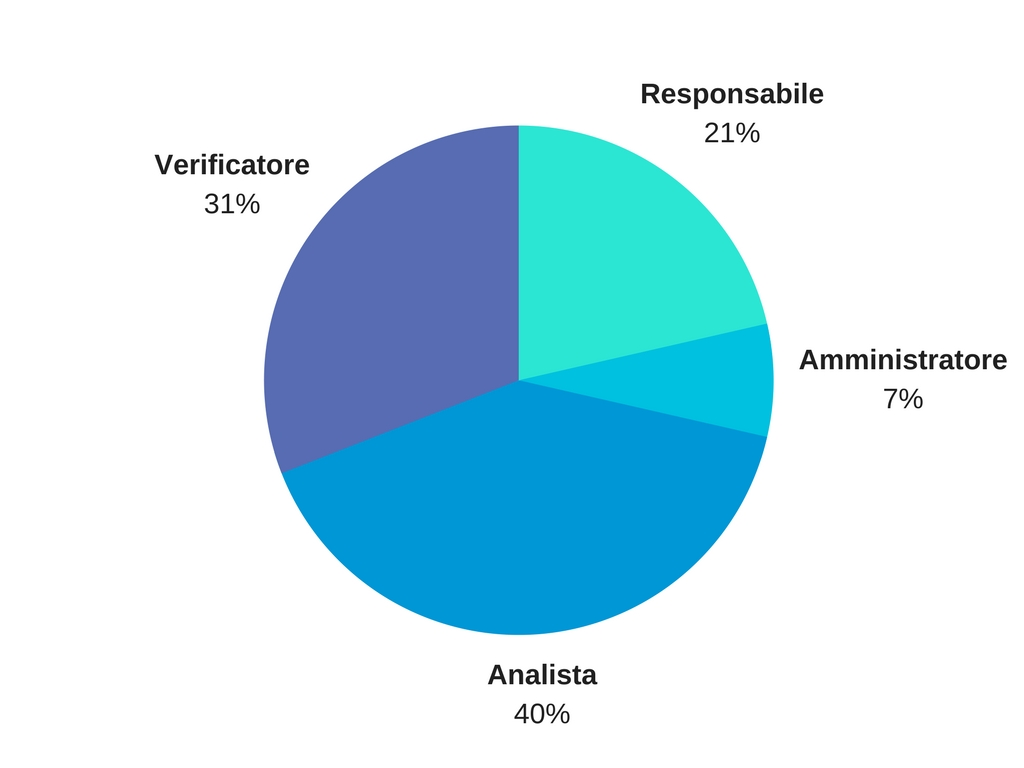
\includegraphics[width=0.9\textwidth]{images/CircolareAnalisiRequisitiDiDettaglio.jpg} 
			\caption{Diagramma circolare ripartizione ore per ruolo - \textit{Analisi dei Requisiti di Dettaglio}}
			\label{CircolareAnalisiRequisitiDiDettaglio}
			\end{figure}
		


		\subsubsection{Progettazione Architetturale}
			\paragraph{Suddivisione lavoro} \Spazio
				Nell'attività di \textit{Progettazione Architetturale} ciascun componente andrà a rivestire i seguenti ruoli:
				\begin{table}[H]
					\centering
					\begin{tabular}{C{4cm}|C{0.6cm}|C{0.6cm}|C{0.6cm}|C{0.6cm}|C{0.6cm}|C{0.6cm}|C{3cm}}
						\hlineB{3}
						\thead{Nominativo} &\thead{Re} &\thead{Am} &\thead{An}&\thead{Pt}&\thead{Pr}&\thead{Ve}&\thead{Ore totali}\\
						\hlineB{3}
						Paolo Eccher & - & - & - & - & - & - & - \\
						Alberto Gallinaro & - & - & - & - & - & - & - \\
						Giuseppe Merlino & - & - & - & - & - & - & - \\
						Elia Montecchio & - & - & - & - & - & - & - \\
						Lisa Parma & - & - & - & - & - & - & - \\
						Francesco Parolini & - & - & - & - & - & - & - \\
						Davide Zago & - & - & - & - & - & - & - \\
						\textbf{Ore totali ruolo}  & \textbf{-} & \textbf{-} & \textbf{-} & \textbf{-} & \textbf{-} & \textbf{-} & \textbf{-} \\
						\hlineB{3}
					\end{tabular}
					\caption{Suddivisione del lavoro - \textit{Progettazione Architetturale}}
				\end{table}
				
			Tali dati sono riassunti graficamente nel seguente diagramma a barre:
			
			\textcolor{red}{METTERE DIAGRAMAM}
							
			\paragraph{Prospetto economico} \Spazio
			Nello svolgimento di questa attività i costi sostenuti per ogni ruolo sono riassunti nella seguente tabella:
			\begin{table}[H]
			\centering
			\begin{tabular}{p{4cm}|C{4cm}|C{4cm}}
				\hlineB{3}
				
				\thead{Ruolo} &\thead{Ore previste} &\thead{Costo}\\
				\hlineB{3}			
				Responsabile & 10 & 300,00\euro \\
				\hline
				Amministratore& 6 & 120,00\euro \\
				\hline
				Analista & - & 0\euro \\
				\hline
				Progettista & 108 & 2376,00\euro \\
				\hline
				Programmatore & - & 0\euro \\
				\hline
				Verificatore & 55 & 825,00\euro \\
				\hline
				\textbf{Ore totali} & \textbf{179} & \textbf{3.621.00 \euro} \\
				\hlineB{3}
			\end{tabular}
			\caption{Costi per ruolo - \textit{Progettazione Architetturale}}
		\end{table}
		
		La ripartizione delle ore tra i vari ruoli è rappresentata graficamente tramite il seguente diagramma circolare:
		
		\begin{figure}[h] 
			\centering 
			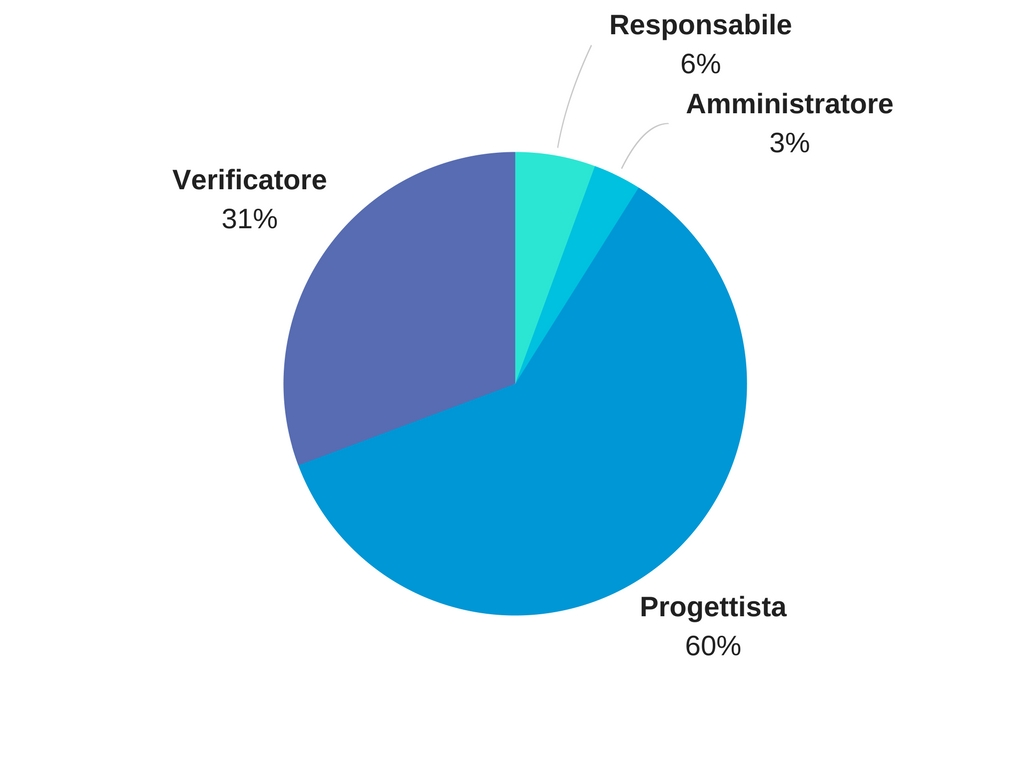
\includegraphics[width=0.9\textwidth]{images/CircolareProgettazioneArchitetturale.jpg} 
			\caption{Diagramma circolare ripartizione ore per ruolo in Progettazione Architetturale}
			\label{CircolareProgettazioneArchitetturale}
		\end{figure}		

		
		\subsubsection{Progettazione di Dettaglio}
			\paragraph{Suddivisione lavoro}
			Nell'attività di \textit{Progettazione di Dettaglio} ciascun componente andrà a rivestire i seguenti ruoli:
			
			\begin{table}[H]
				\centering
				\begin{tabular}{C{4cm}|C{0.6cm}|C{0.6cm}|C{0.6cm}|C{0.6cm}|C{0.6cm}|C{0.6cm}|C{3cm}}
					\hlineB{3}
					\thead{Nominativo} &\thead{Re} &\thead{Am} &\thead{An}&\thead{Pt}&\thead{Pr}&\thead{Ve}&\thead{Ore totali}\\
					\hlineB{3}
					Paolo Eccher & - & - & - & - & - & - & - \\
					Alberto Gallinaro & - & - & - & - & - & - & - \\
					Giuseppe Merlino & - & - & - & - & - & - & - \\
					Elia Montecchio & - & - & - & - & - & - & - \\
					Lisa Parma & - & - & - & - & - & - & - \\
					Francesco Parolini & - & - & - & - & - & - & - \\
					Davide Zago & - & - & - & - & - & - & - \\
					\textbf{Ore totali ruolo}  & \textbf{-} & \textbf{-} & \textbf{-} & \textbf{-} & \textbf{-} & \textbf{-} & \textbf{-} \\
					\hlineB{3}
				\end{tabular}
				\caption{Suddivisione del lavoro - \textit{Progettazione di Dettaglio}}
			\end{table}
			
			Tali dati sono riassunti graficamente nel seguente diagramma a barre:
			
			\textcolor{red}{METTERE DIAGRAMAM}
			
			\paragraph{Prospetto economico} \Spazio
			Nello svolgimento di questa attività i costi sostenuti per ogni ruolo sono riassunti nella seguente tabella:
			\begin{table}[H]
			\centering
			\begin{tabular}{p{4cm}|C{4cm}|C{4cm}}
				\hlineB{3}
				
				\thead{Ruolo} &\thead{Ore previste} &\thead{Costo}\\
				\hlineB{3}			
				Responsabile & 8 & 240,00\euro \\
				\hline
				Amministratore& 7 & 140,00\euro \\
				\hline
				Analista & - & 0\euro \\
				\hline
				Progettista & 95 & 2.090,00\euro \\
				\hline
				Programmatore & - & 0\euro \\
				\hline
				Verificatore & 53 & 795,00\euro \\
				\hline
				\textbf{Ore totali} & \textbf{163} & \textbf{3.265,00 \euro} \\
				\hlineB{3}
			\end{tabular}
			\caption{Costi per ruolo - \textit{Progettazione di Dettaglio}}
		\end{table}
		
		La ripartizione delel ore tra i vari ruoli è rappresentata graficamente tramite il seguente diagramma circolare:
		
		\begin{figure}[h] 
			\centering 
			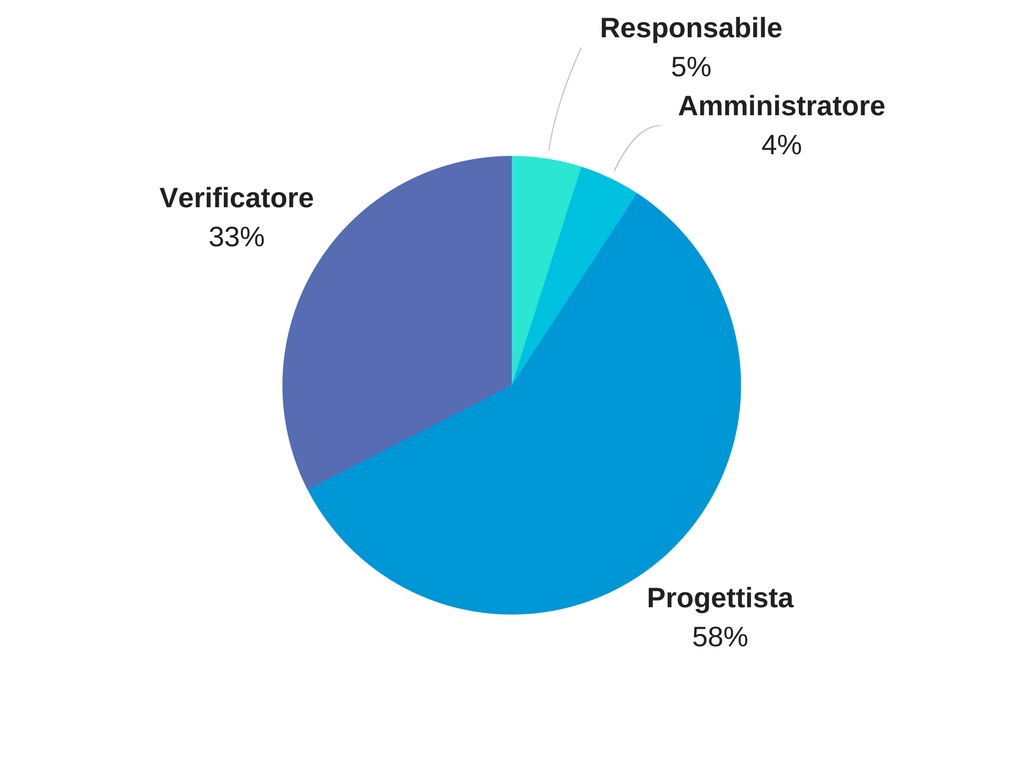
\includegraphics[width=0.9\textwidth]{images/CircolareProgettazioneDiDettaglio.jpg} 
			\caption{Diagramma circolare ripartizione ore per ruolo in Progettazione di Dettaglio}
			\label{CircolareProgettazioneDiDettaglio}
		\end{figure}		
		
		
		\subsubsection{Codifica}
			\paragraph{Suddivisione lavoro}
			Nell'attività di \textit{Codifica} ciascun componente andrà a rivestire i seguenti ruoli:
			\begin{table}[H]
				\centering
				\begin{tabular}{C{4cm}|C{0.6cm}|C{0.6cm}|C{0.6cm}|C{0.6cm}|C{0.6cm}|C{0.6cm}|C{3cm}}
					\hlineB{3}
					\thead{Nominativo} &\thead{Re} &\thead{Am} &\thead{An}&\thead{Pt}&\thead{Pr}&\thead{Ve}&\thead{Ore totali}\\
					\hlineB{3}
					Paolo Eccher & - & - & - & - & - & - & - \\
					Alberto Gallinaro & - & - & - & - & - & - & - \\
					Giuseppe Merlino & - & - & - & - & - & - & - \\
					Elia Montecchio & - & - & - & - & - & - & - \\
					Lisa Parma & - & - & - & - & - & - & - \\
					Francesco Parolini & - & - & - & - & - & - & - \\
					Davide Zago & - & - & - & - & - & - & - \\
					\textbf{Ore totali ruolo}  & \textbf{-} & \textbf{-} & \textbf{-} & \textbf{-} & \textbf{-} & \textbf{-} & \textbf{-} \\
					\hlineB{3}
				\end{tabular}
				\caption{Suddivisione del lavoro - \textit{Codifica}}
			\end{table}
			
			Tali dai sono riassunti graficamente nel seguente diagramma a barre:
			
			\textcolor{red}{METTERE DIAGRAMAM}
			
			
			\paragraph{Prospetto economico} \Spazio
			Nello svolgimento di questa attività i costi sostenuti per ogni ruolo sono riassunti nella seguente tabella:
			\begin{table}[H]
				\centering
				\begin{tabular}{p{4cm}|C{4cm}|C{4cm}}
					\hlineB{3}
					
					\thead{Ruolo} &\thead{Ore previste} &\thead{Costo}\\
					\hlineB{3}			
					Responsabile & 11 & 330,00\euro \\
					\hline
					Amministratore& 6 & 120,00\euro \\
					\hline
					Analista & - & 0\euro \\
					\hline
					Progettista & 27 & 594,00\euro \\
					\hline
					Programmatore & 117 & 1.755,00\euro \\
					\hline
					Verificatore & 74 & 1.110,00\euro \\
					\hline
					\textbf{Ore totali} & \textbf{235} & \textbf{3.909,00 \euro} \\
					\hlineB{3}
				\end{tabular}
					\caption{Costi per ruolo - \textit{Codifica}}
			\end{table}
			
			La ripartizione delle ore tra i vari ruoli è rappresentata graficamente tramite il seguente diagramma circolare:

		\begin{figure}[h!] 
			\centering 
			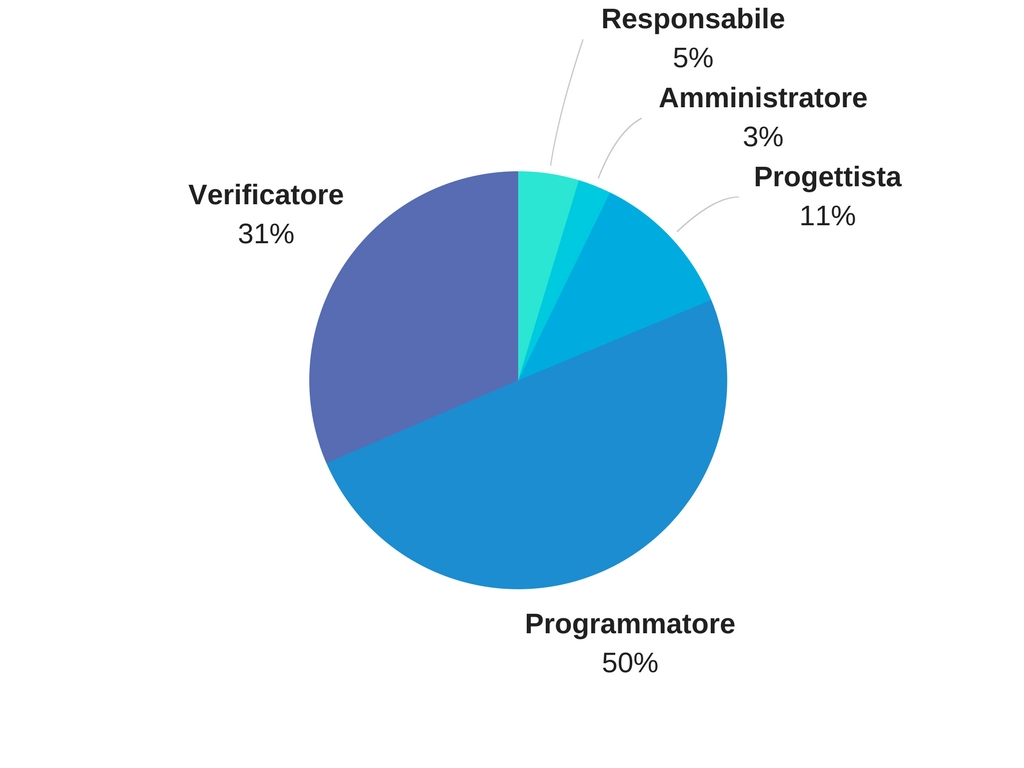
\includegraphics[width=0.9\textwidth]{images/CircolareCodifica.jpg} 
			\caption{Diagramma circolare ripartizione ore per ruolo in Codifica}
			\label{CircolareCodifica}
		\end{figure}
	
		\subsubsection{Verifica Validazione}
			\paragraph{Suddivisione lavoro}
			\paragraph{Prospetto economico}			
	\subsection{Riepilogo}
		\subsubsection{Ore totali di investimento}
			\paragraph{Suddivisione lavoro} \Spazio
			Il totale delle ore investite, consideranto sia quelle rendicontate che quelle d'investimento non redicontate sono riassunte nella seguente tabella:
					\begin{table}[H]
			\centering
			\begin{tabular}{C{4cm}|C{0.6cm}|C{0.6cm}|C{0.6cm}|C{0.6cm}|C{0.6cm}|C{0.6cm}|C{3cm}}
				\hlineB{3}
				\thead{Nominativo} &\thead{Re} &\thead{Am} &\thead{An}&\thead{Pt}&\thead{Pr}&\thead{Ve}&\thead{Ore totali}\\
				\hlineB{3}
				Paolo Eccher & - & - & - & - & - & - & - \\
				Alberto Gallinaro & - & - & - & - & - & - & - \\
				Giuseppe Merlino & - & - & - & - & - & - & - \\
				Elia Montecchio & - & - & - & - & - & - & - \\
				Lisa Parma & - & - & - & - & - & - & - \\
				Francesco Parolini & - & - & - & - & - & - & - \\
				Davide Zago & - & - & - & - & - & - & - \\
				\textbf{Ore totali ruolo}  & \textbf{-} & \textbf{-} & \textbf{-} & \textbf{-} & \textbf{-} & \textbf{-} & \textbf{-} \\
				\hlineB{3}
			\end{tabular}
			\caption{Suddivisione del lavoro - Investimento totale }
			\end{table}
		
			Tali dati sono riassunti graficamente nel seguente diagramma a barre:
			
			\textcolor{red}{DIAGRAMAM}
			
			La ripartizione delle ore tra i vari ruoli è rappresentata graficamente 
			attraverso il seguente diagramma circolare:
			
			\textcolor{red}{DIAGRAMAM}
			
			\subsubsection{Ore Rendicontate}
			
			\paragraph{Suddivisione lavoro} \Spazio
			Le ore rendicontate sono riassunte nella seguente tabella:
			\begin{table}[H]
				\centering
				\begin{tabular}{C{4cm}|C{0.6cm}|C{0.6cm}|C{0.6cm}|C{0.6cm}|C{0.6cm}|C{0.6cm}|C{3cm}}
					\hlineB{3}
					\thead{Nominativo} &\thead{Re} &\thead{Am} &\thead{An}&\thead{Pt}&\thead{Pr}&\thead{Ve}&\thead{Ore totali}\\
					\hlineB{3}
					Paolo Eccher & - & - & - & - & - & - & - \\
					Alberto Gallinaro & - & - & - & - & - & - & - \\
					Giuseppe Merlino & - & - & - & - & - & - & - \\
					Elia Montecchio & - & - & - & - & - & - & - \\
					Lisa Parma & - & - & - & - & - & - & - \\
					Francesco Parolini & - & - & - & - & - & - & - \\
					Davide Zago & - & - & - & - & - & - & - \\
					\textbf{Ore totali ruolo}  & \textbf{-} & \textbf{-} & \textbf{-} & \textbf{-} & \textbf{-} & \textbf{-} & \textbf{-} \\
					\hlineB{3}
				\end{tabular}
				\caption{Suddivisione del lavoro - Ore rendicontate }
			\end{table}
			
			Tali dati sono riassunti graficamente nel seguente diagramma a barre:
			
			\textcolor{red}{DIAGRAMAM}
			
			\paragraph{Prospetto economico} \Spazio
			Il totale rendicontato dei costi sostenuti per ogni ruolo è riassunto nella seguente tabella:
			\begin{table}[H]
				\centering
				\begin{tabular}{p{4cm}|C{4cm}|C{4cm}}
					\hlineB{3}
					
					\thead{Ruolo} &\thead{Ore previste} &\thead{Costo}\\
					\hlineB{3}			
					Responsabile & 11 & 330,00\euro \\
					\hline
					Amministratore& 6 & 120,00\euro \\
					\hline
					Analista & - & 0\euro \\
					\hline
					Progettista & 27 & 594,00\euro \\
					\hline
					Programmatore & 117 & 1.755,00\euro \\
					\hline
					Verificatore & 74 & 1.110,00\euro \\
					\hline
					\textbf{Ore totali} & \textbf{235} & \textbf{3.909,00 \euro} \\
					\hlineB{3}
				\end{tabular}
				\caption{Costi per ruolo - Ore rendicontate}
			\end{table}
		
			La ripartizione delle ore tra i vari ruoli è rappresentata graficamente attraverso il seguente diagramma circolare:
			\textcolor{red}{DIAGRAMAM}
			
			\subsubsection{Conclusioni}
			
			Il costo totale preventivato per il progetto è -----------
